%% USPSC-Cap3-Conclusao.tex
% ---
% Conclusão
% ---
\chapter{Resultados}

Para gerar um \textit{Dashboard} o usuário precisa definir o escopo na extração, o código, na linguagem R, permite a escolha da janela de tempo e unidades federativas a serem analisadas, com base na biblioteca desenvolvida por \citeonline{saldanha2019microdatasus}, atualmente não existe uma interface para sta escolha, a alteração é feita diretamente no código, adicionalmente a extração é feita no mesmo ambiente.

Um \textit{Dashboard} foi elaborado com seu design voltado para a exploração dos dados de forma sequencial, a primeira página (ver \autoref{fig_dash_1}) permite uma visão geográfica, onde é possível filtrar unidades federativas e municípios, além de permitir selecionar o filtro `Reduzíveis', este filtro representa a forma de prevenção que pode reduzir a causa de morte associada, a relação foi construída com base na lista elaborada por \citeonline{malta2007causas}, após o filtro é possível observar o mapa, que indica a localização geográfica da morte e os códigos CID associados na legenda, este \textit{Dasboard} contem a contagem das mortes está disponível, que é alterada de forma dinâmica, em relação aos filtros selecionados.

\begin{figure}[H]
	\caption{\label{fig_dash_1}Página 1 do \textit{Dashboard} com filtros aplicados}
	\begin{center}
		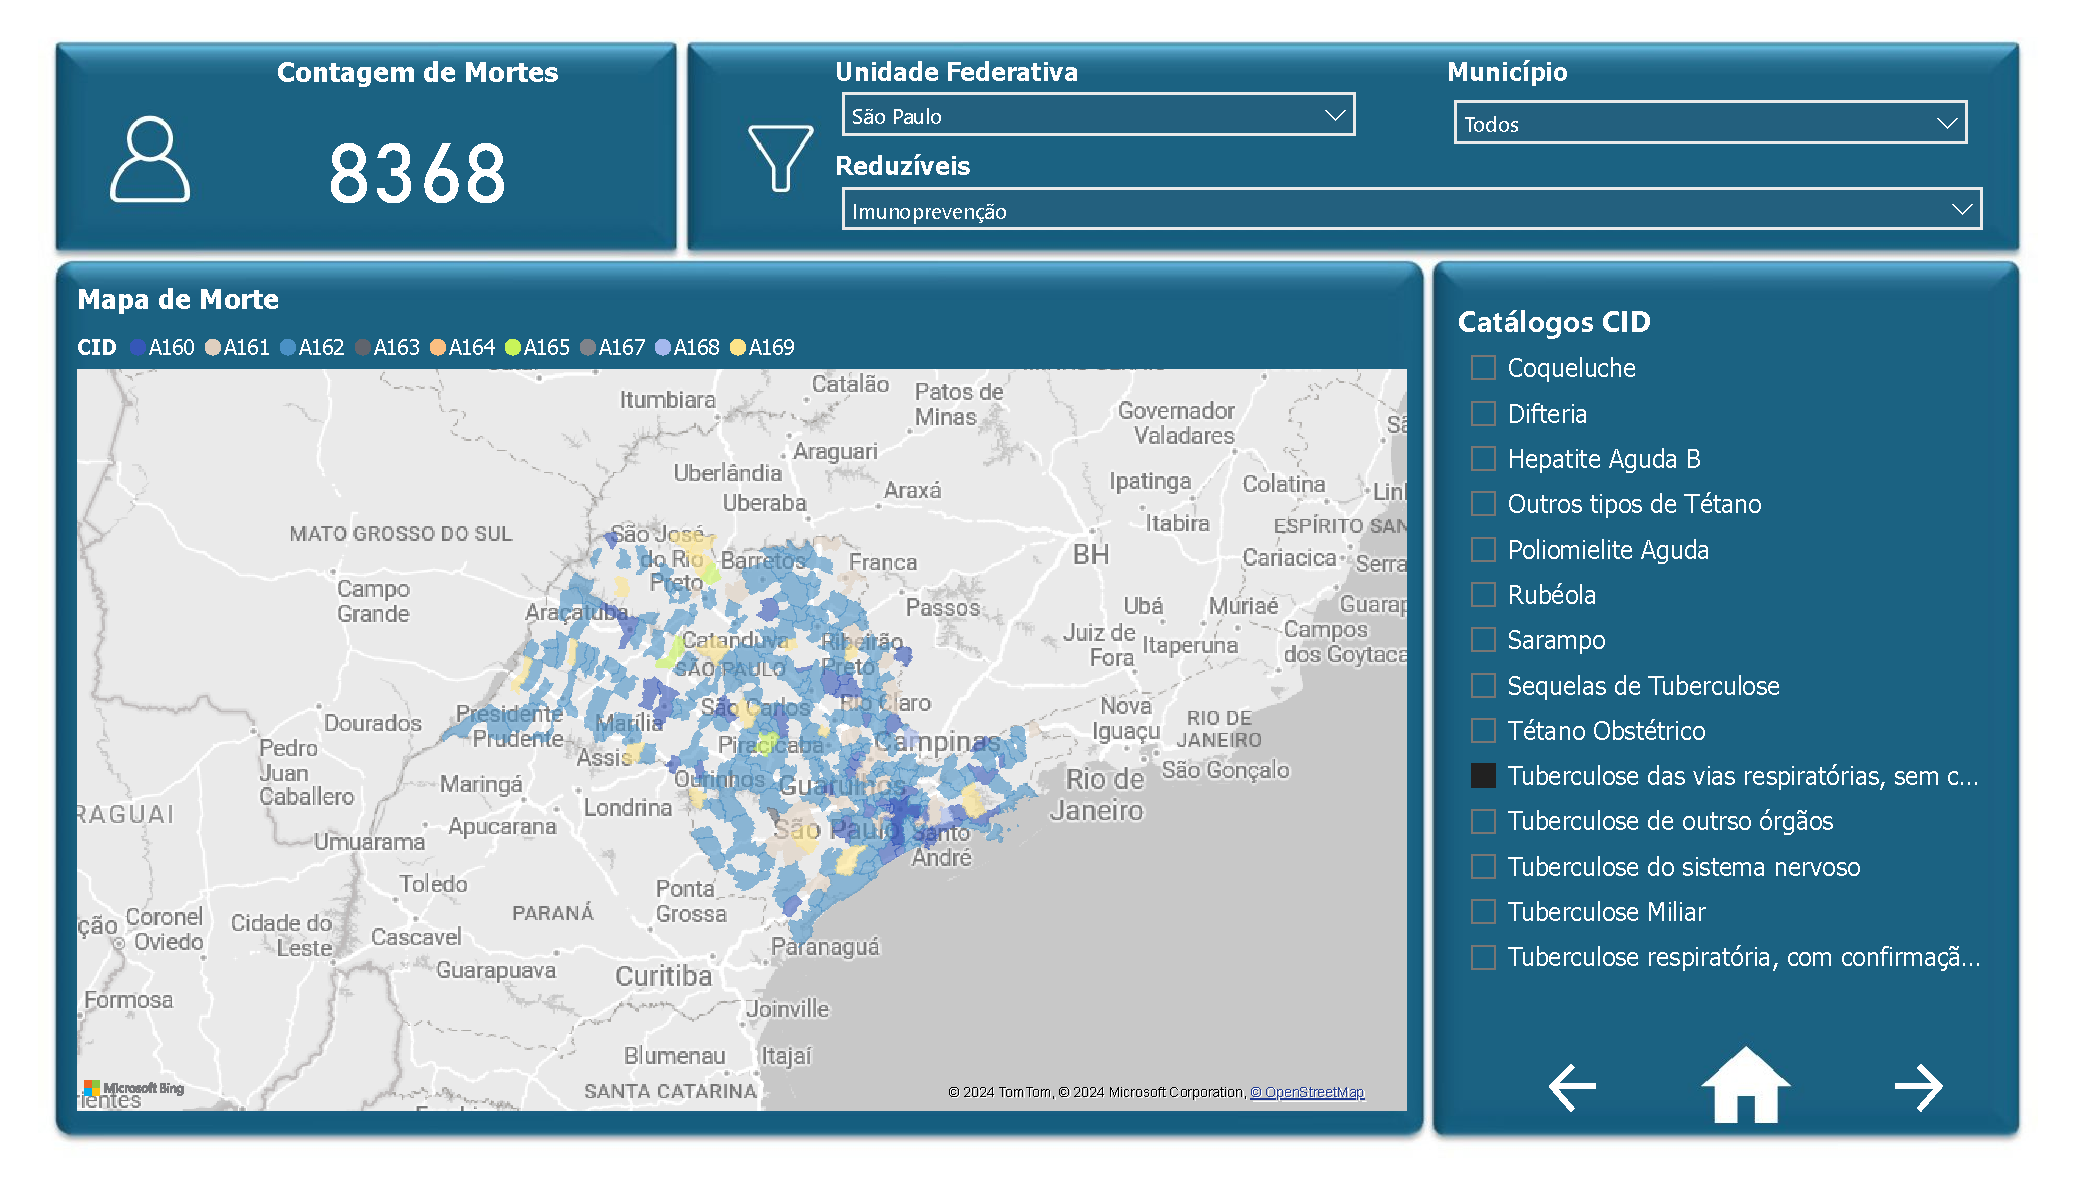
\includegraphics[width=\textwidth, page = 1]{USPSC-img/dash}
	\end{center}
	\legend{Fonte: SIM-DO e Resultados da Pesquisa}
\end{figure}

A segunda página proporciona uma visão temporal e por sexo (ver \autoref{fig_dash_2}), os filtros de unidade federativa, município e `Reduzíveis', após a seleção dos filtros desejados as informações de quantidades de mortes por sexo, cidade, ano e causa da morte, esta visão possibilita a observação sobre a evolução temporal, além de permitir a visão sobre as causas mais frequentes. A ferramenta \textit{PowerBI} também permite ao usuário que se utilize do próprio gráfico para filtragem, como exemplo, caso o usuário selecione o sexo masculino do gráfico o \textit{Dashboard} sera filtrado e adaptado de acordo.

\begin{figure}[H]
	\caption{\label{fig_dash_2}Página 2 do \textit{Dashboard} com filtros aplicados}
	\begin{center}
		\includegraphics[width=\textwidth, page = 2]{USPSC-img/dash}
	\end{center}
	\legend{Fonte: SIM-DO e Resultados da Pesquisa}
\end{figure}

A terceira e quarta página permitem uma visão analítica com base em faixa etária (ver \autoref{fig_dash_3}), de acordo com a definição da Organização Mundial de Saúde (OMS), e pelo campo RACACOR disponível nos dados, definidas como Raça/Cor (ver \autoref{fig_dash_3}). Ambos os casos permitem filtros de unidade federativa, municípios e `Reduzíveis', além de permitir um corte temporal pela escolha de um intervalo por data de óbito.

\begin{figure}[H]
	\caption{\label{fig_dash_3}Página 3 do \textit{Dashboard} com filtros aplicados}
	\begin{center}
		\includegraphics[width=\textwidth, page = 3]{USPSC-img/dash}
	\end{center}
	\legend{Fonte: SIM-DO e Resultados da Pesquisa}
\end{figure}

\begin{figure}[H]
	\caption{\label{fig_dash_4}Página 4 do \textit{Dashboard} com filtros aplicados}
	\begin{center}
		\includegraphics[width=\textwidth, page = 4]{USPSC-img/dash}
	\end{center}
	\legend{Fonte: SIM-DO e Resultados da Pesquisa}
\end{figure}

É importante ressaltar que as mortes de pessoas brancas representam 73\% das causas, este é um número a ser considerado com cautela, dado a problemática envolvendo o preenchimento dos dados apontado por \citeonline{muzy2021analise}, desta forma conclusões sobre mortes em relação a Raça/Cor devem levar em conta esta deficiência na coleta dos dados. Todos os códigos desenvolvidos neste trabalho estão disponíveis em um repositório público \cite{lucas_barbosa_defanti_2024_11526926}.


